\documentclass{article}

% Formatting
\usepackage[utf8]{inputenc}
\usepackage[margin=1in]{geometry}
\usepackage[titletoc,title]{}

% Math
% https://www.overleaf.com/learn/latex/Mathematical_expressions
% https://en.wikibooks.org/wiki/LaTeX/Mathematics
\usepackage{amsmath,amsfonts,amssymb,mathtools}

% Images
% https://www.overleaf.com/learn/latex/Inserting_Images
% https://en.wikibooks.org/wiki/LaTeX/Floats,_Figures_and_Captions
\usepackage{graphicx,float}   % needed for figures
\usepackage{subcaption}

% Tables
% https://www.overleaf.com/learn/latex/Tables
% https://en.wikibooks.org/wiki/LaTeX/Tables
\usepackage{tabularx}

% Algorithms
% https://www.overleaf.com/learn/latex/algorithms
% https://en.wikibooks.org/wiki/LaTeX/Algorithms
\usepackage[ruled,vlined]{algorithm2e}
\usepackage{algorithmic}

% Code syntax highlighting
% https://www.overleaf.com/learn/latex/Code_Highlighting_with_minted
\usepackage{minted}
\usemintedstyle{borland}

% References
% https://www.overleaf.com/learn/latex/Bibliography_management_in_LaTeX
% https://en.wikibooks.org/wiki/LaTeX/Bibliography_Management
\usepackage{biblatex}
\addbibresource{references.bib}

% to be able to click on links and references
\usepackage{hyperref}


% Title content
\title{Computational Physics II - Project 2 \\ Time Independent Schrödinger Equation in 1D}
\newcommand{\aone}{Adrian Stroth}
\newcommand{\atwo}{Edoardo Stefanin Mustacchi}
\newcommand{\athree}{Francisco Crespo}
\newcommand{\afour}{Cabibbo Group}
\author{\aone\space, \atwo\space and \athree \\ \afour}
\date{\today}

\begin{document}

\maketitle
\tableofcontents
\begin{abstract}
 
\end{abstract}

%  Code intallation & verification
\section{Code - TISE}\label{code}
The code described in this report simulates a quantum mechanical system in 1D. It approximates the groundstate and its energy of an one dimensional Schr\"{o}dinger equation (SEQ). 
Additionally, it calculates the average position and momentum, standard deviation of position and momentum and average kinetic, potential and state energy. 
Four possible choices in potentials are provided; zero potential, harmonic potential, well potential and wall potential. Moreover, the size of the simulated system L can be chose for each simulation. 
To solve the SEQ computationally, the system was discretized. 
This means the system corresponds to a number of points with size $L = AxN$ with A being the lattice spacing and N the number of lattice points. A can be chosen with the discretized mass $\hat{m} = \frac{m \varepsilon a^2}{\hbar^2}$. 
This code works with $m = \varepsilon = \hbar = 1$ as the desired physical values can be implemented into the codes output in postprocessing.
This results in the two dimensionless parameters N and $\hat{m}$ and the potential choice to initialize the desired system. 
The number of lattice points is counted from 0 to N-1 with the requirements $N<0$ and N odd. 
This way the center of the system lies on a lattice point.
The parameters L and A have to be chosen by thoughtful adjust of N and m. \\
\\
Most of the code is written in c and bash scripts are provided to compile the files and run the simulations as the code is structured in a modular fashion.
The three main modules {\fontfamily{qcr}\selectfont hamiltonian.c, powermethod.c} and {\fontfamily{qcr}\selectfont conjugategradient.c} make up most of the code and work independently of each other. They are supported by the smaller modules {\fontfamily{qcr}\selectfont assert.c, wavefunction.c, geometry.c linearalgebra.c} and {\fontfamily{qcr}\selectfont observables.c}.\\

% subsection hamiltonian 
\subsection{Hamiltonian}\label{hmltn}
This module is the quantum mechanical heart of the code. It initializes the parameters $\hat{m}$, N and the potential and builds the corresponding Hamiltonian.

It thereby uses a discretized second derivative in the kinetic energy, with the use of Dirichlet boundary conditions.
With this implemention of a finite derivative the resulting matrix will be sparse. Therefore the hamiltonian itself is never stored as a matrix but but instead the {\fontfamily{qcr}\selectfont hamiltonian.c} module contains a function which computes the vector to which the Hamiltonian was applied
Main choices of this module are:
\begin{itemize}
    \item $m = \varepsilon = \hbar = 1$
    \item the discretized second derivative $\hat{\psi}(n) = \hat{\psi}(n+1)-2\hat{\psi}(n)+\hat{\psi}(n-1))$
    \item Dirichlet boundary conditions: $\hat{\psi}(0-1)=0$ and $\hat{\psi}(N-1+1)=\hat{\psi}(N)=0$
    \item four possible potentials 
\end{itemize}
The four possible potential numbered 0 to 3 are
\begin{itemize}
    \item a zero potential that sets all potential values on the lattice points to zero,
    \item a harmonic potential ...   ,
    \item a well potential, which is placed in the system's center, has a length of N/2 and is 0 in the well and 1 outside of it, 
    \item a wall potential, that begins at N+1/2 and has a height of 1.
\end{itemize}
Additionally, {\fontfamily{qcr}\selectfont hamiltonian.c} can set the Hamiltonian to be positive definite and calculate and return the average kinetic, potential and state energy of a given wavefunction.\\
\\
This module is tested with the files {\fontfamily{qcr}\selectfont analytic.c, hermitian.c, linearity.c} . 
\begin{itemize}
    \item In {\fontfamily{qcr}\selectfont analytic.c} the potential is set to be null. The eigenvectors then can be analytically determined. Since the Dirichlet Boundary conditions forces the wavefunction to have eigenvectors of the form
    
    
    
    $\psi(n) = sin(\frac{\pi(n+1)k}{N+1})$
    
    
    Where k gives the k-th eigenvector.
    This test is used to check whether the discretized derivative produces sensible results. Here the tolerance is taken to be $1e^{-15}$
    
    \item In {\fontfamily{qcr}\selectfont linearity.c} one of the two basic physical properties of the hamiltonian is tested: its linearity. 
    Two random wave functions are generated, then two more complex coefficients.
    Then the two terms of the equivalence relation
    % $$ $$ sets the formuala in an independet own line and $ $ keeps it in the line it is written 
    $$
    \hat{H}(\alpha_1\hat{\psi_1} + \alpha_2\psi_2)  = \alpha_1(\hat{H}\hat{\psi_1} + \alpha_2(\hat{H}\hat{\psi_2})
    $$
    
    Are computed separately, subtracted and the norm of the resulting vector is taken to provide a good estimation of the error. In this routine it is possible to input different parameters including the type of potential that the user wishes to have and the tolerance parameter. The linearity has been verified with a tolerance factor up to $10^-15$
    
    \item At last the hermiticity of the hamiltonian is put to the test with a procedure similar to that of linearity.
    The two sides of the equivalence equation 
    $$ (\hat{\psi_1}, \hat{H}\hat{\psi_2}) = (\hat{H}\hat{\psi_1},\hat{\psi_2})$$
    
    Are computed, the distance between the two values is then computed. It is possible to fix the desired tolerance and choice of potential.
    
\end{itemize}

% subsection power method  
\subsection{Power Method}\label{pwr mthd}
The power method is a method that computes the largest eigenvalue and its corresponding eigenvector of a given matrix definite positive linear transformation M. 
It is an iterative algorithm, that was implemented as described in the project description.
Its inputs are the desired tolerance which is the stopping criteria, a complex output vector and a function with input and output vector that calculates a linear transformation M applied on the input vector.

Inside the power method a random complex array pf the form $w_0 = random\_a + i * random\_b$ is created.
This vector is given to the aforementioned function.
By iterating through the algorithm the vector $\Bar{w}$ corresponding to the largest eigenvalue $\mu$ is approximated.
% if time insert formula
The power method write this vector onto the given output vector and returns the eigenvalue.\\
\\
Testing of the power method is performed via {\fontfamily{qcr}\selectfont power\_algo.c} in the test directory.
It creates a random positive semi definite matrix $M=A^{\dagger}A$ and calculates its largest eigenvalue and the corresponding eigenvector.
It estimates 
$$ || Mw -\mu w|| < \epsilon $$

And prints out the result. A test is considered passed if the distance between the two vectors is smaller than the tolerance chosen. 

\\
\\

%subsection conjugate gradient 
\subsection{Conjugate Gradient}\label{cnjgt grdnt}
The conjugate gradient module is used to calculate the inverse of the Hamiltonian.
As the power method retrieves the largest eigenvalue it is fed the inverse of a matrix to calculate the smallest eigenvalue.
Therefore, the conjugate gradient method is used to provide the function for the power method.
This module then approximates $M^{-1}v$ for every positive definite matrix M and any vector v. It approximates the solution to the equation $Mx=b$.
As input it takes two complex vectors x and b and a function that represents the matrix M and calculates $Mv$.
This function has to be positive definite.
The stopping criteria is set inside the module by the residue, that is given as input parameter to the code.
Inside the module this is called the accuracy.
As suggested in the project description, the algorithm was implemented as demonstrated on the conjugate gradient wikipedia page.\\
\\
To test this module the {\fontfamily{qcr}\selectfont test\_conjugate.c} code is used.
This test creates a random positive definite matrix M and applies the conjugate gradient method to generate $M^{-1}b = x$.
Then $Mx=b$ is calculated to check if the output . % THIS IS PROBABLY WRONG
To compare the results and approve the test, all matrices are printed to the console.\\
\\


\subsection{Main code}\label{main}
The goal of this code is to use the power method and conjugate gradient to calculate the groundstate energy and gound state wavefunction of a given hamiltonian. 
Thus the structure of the main.c is as follows:
\begin{enumerate}
    \item The input parameters N, mass (meaning $\hat{m}$), potential choice, tolerance and residue are read in from the console and set.
    \item The Hamiltonian is initialized and made positive definite.
    \item An eigenstate and eigenvalue are initialized.
    \item The power method is called with the eigenstate and the conjugate gradient. Since the conjugate gradient takes different inputs than required by the power method, a wrapper function called {\fontfamily{qcr}\selectfont H\_inv()} that calls conjugate gradient is used.
    \item The eigenvalue is calculated from the returned eigenvalue an subtracting or adding the constant that was used to make H positive definite.
    \item Various observables are calculated and printed to output files.
\end{enumerate}
In total the simulation creates three output files in the output directory: {\fontfamily{qcr}\selectfont ES\_values.txt, observ\_values.txt} and {\fontfamily{qcr}\selectfont input\_parameters\_values.txt}. They contain the eigenstate values, the observables and the chosen input parameters, respectively.\\
\\
%subsection other modules 
\subsection{Side Modules}
A description of the other modules that support the main simulation is presented in the folllowing.
\begin{itemize}
    \item {\fontfamily{qcr}\selectfont assert.c}: this module provided by professor Patella can be used to check that the right amount of parameters are passed by the user and a tailored error can be printed if they are not
    \item {\fontfamily{qcr}\selectfont wavefunction.c}: This module can create a random normalized wavefunction.
    \item {\fontfamily{qcr}\selectfont geomerty.c}: This module sets the geometry parameter of the system N, which is implemented as constant global variable. It also contains a function to return N.
    \item {\fontfamily{qcr}\selectfont linearalgebra.c}: This modules contains functions that can calculate a scalarproduct of two complex vectors and given size and a function to calculate the norm of a given vector with given size.
    \item {\fontfamily{qcr}\selectfont observables.c}: This modules contains functions that calculate and return the average position, average momentum and standard deviation of the position and momentum of a given wavefunction.
\end{itemize}
%
%subsection compiling and running 
\subsection{Compiling and Running of the Code}
After downloading the code from \ref{code} on should have the necessary directory structure saved locally.
To compile all files on runs the script {\fontfamily{qcr}\selectfont compile.sh} from within TISE directory.
This creates a {\fontfamily{qcr}\selectfont main.o} inside TISE and executables of every test program inside the test directory.
Afterwards there exist two ways to run simulations. 
\begin{enumerate}
    \item Run from within TISE \begin{verbatim}
        main.o [N] [mass] [potential] [tolerance] [residue]
    \end{verbatim}
    \item Enter the desired parameters for simulation or many simulations in the {\fontfamily{qcr}\selectfont run\_simulation.sh} script and run from within TISE 
        \begin{verbatim}
            ./scripts/run_simulation.sh
        \end{verbatim} 
        or run the script from within scripts.
\end{enumerate}

% section Algorithmic params
\section{Study of the algorithmic parameters}\label{algrmtc parmtrs}
What is the idea behind that?
Why do we want to study the parameters?
What are we expecting to see?\\

\subsection{Effect of tolerance on power method}
Table with the testing systematic (the parameters that were used as inputs, the potentials we are testing)\\
Parameters to study: stability of the wave function, average total energy, average kinetic and potential energies, average position and momentum, standard deviation of position and momentum\\
for a couple of potentials\\
Results: How did we see the results (or could we show some plot)? What is our conclusion or why and how do we decide on a successful test.\\
We should have plots for the energy and observables and also wave function!!\\

\subsection{Effect of residue on conjugate gradient}
Table with the testing systematic (the parameters that were used as inputs)\\
Parameters to study: stability of the wave function, average total energy, average kinetic and potential energies, average position and momentum, standard deviation of position and momentum\\
for a couple of potentials\\
Results: How did we see the results (or could we show some plot)? What is our conclusion or why and how do we decide on a successful test.\\
We should have plots for the energy and observables and also wave function!!\\

\section{Continuum Limit}\label{finitevol}
Theory and what we expect to happen. \\
What parameters to we change to study the effects? \\
For only one potential\\

Show resulting plots.\\
Talk about the result, what are out conclusions? \\
% Example of how to include plots
\begin{figure}
    \centering
    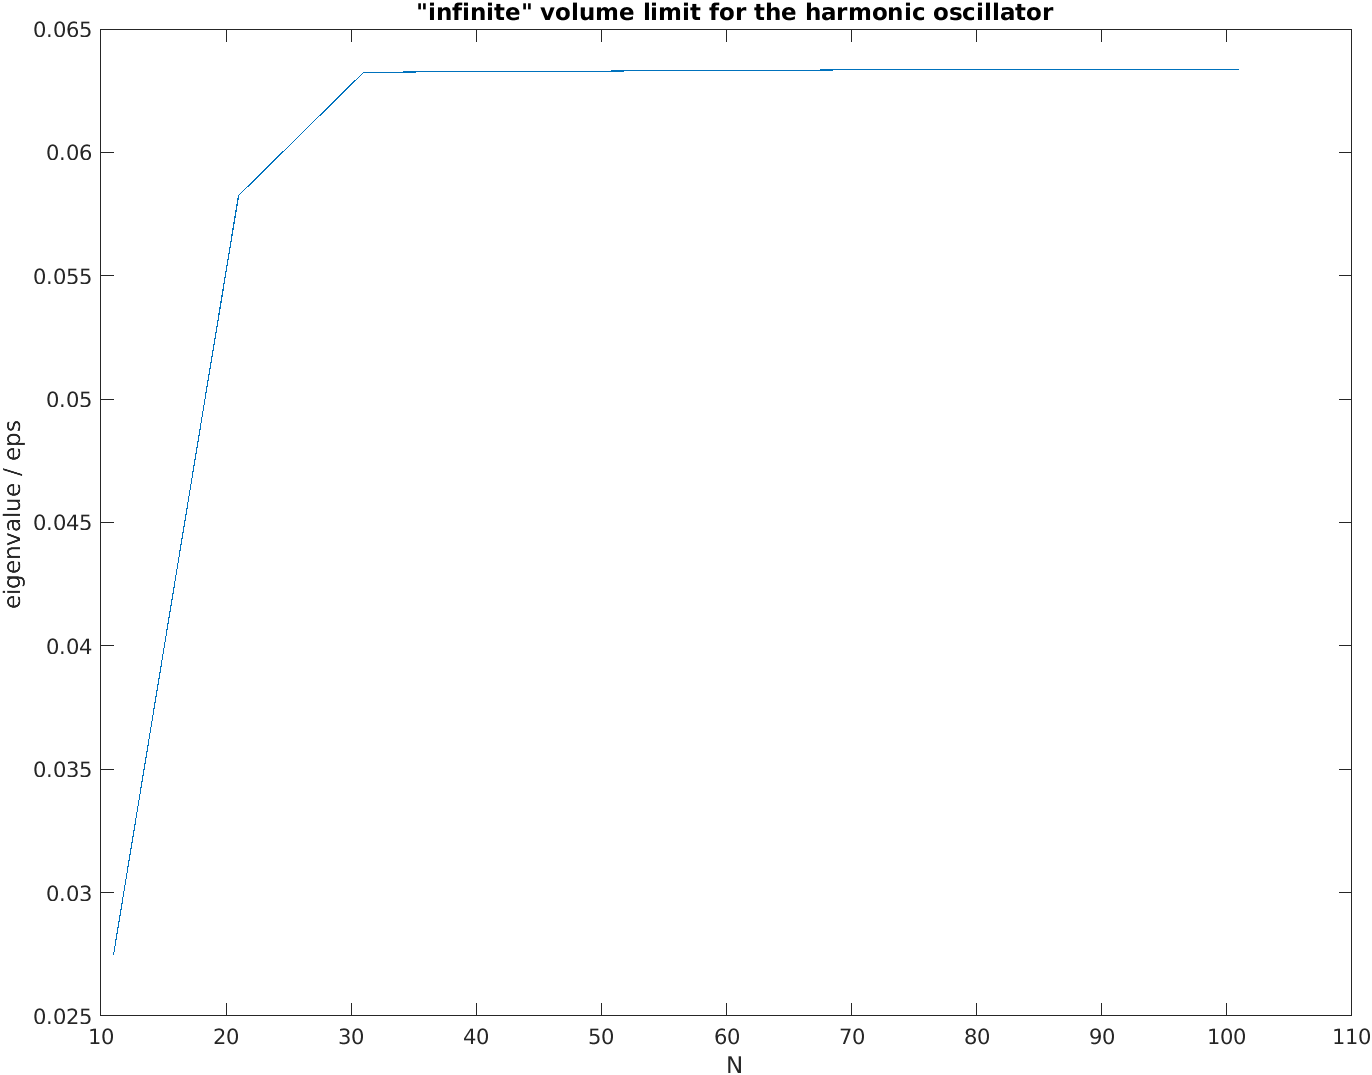
\includegraphics[scale = 0.7]{inf_volume_limit}
    \caption{While keeping the parameter m constant, as well as all the other parameters, we varied the number of lattice points N. N}
    \label{a0(1/A)}
\end{figure}


\clearpage
\section{Additional notes}
Link to the code: \hyperlink{https://github.com/carlulli/TISE}{Code}.

%\printbibliography
\end{document}
